\section{Symbolic Regression: Example Problem}
At first we discuss a case study which is an extended version of the multivalued symbolic regression problem provided as an tutorial for ECJ (Evolutionary Computation in Java)\footnote{\url{https://cs.gmu.edu/~eclab/projects/ecj/docs/tutorials/tutorial4/index.html}}. 

\subsection{Representation}
In the symbolic regression problem, there are six nodes representing the terminals nodes \textbf{X} and \textbf{Y}, and the function nodes \textbf{add} (+), \textbf{sub} (-), \textbf{mul} (*), and \textbf{div} (/). 
\begin{figure}
	\centering
	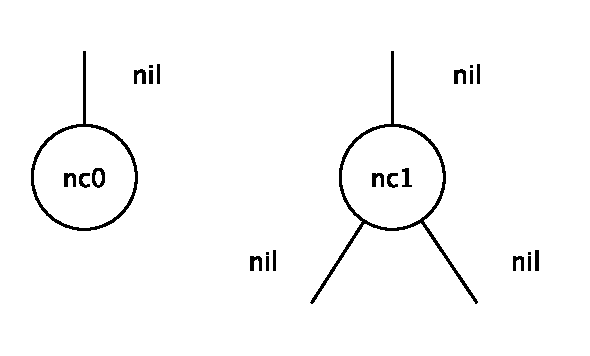
\includegraphics[width=0.5\linewidth]{./fig/symbolic_example_ncs}
	\caption{Node constraints for the symbolic regression problem.}
	\label{fig:symb_ncs}
\end{figure}

The terminal nodes conform to the node constraint \emph{nc0}, and the function nodes conform to the node constraint \emph{nc1} in Figure~\ref{fig:symb_ncs}. \emph{nc0} specifies that nodes which conform to it (Nodes \textbf{X} and \textbf{Y}) should have their return types as \emph{nil}, which is ECJ's default type. \emph{nc0} nodes should have 0 children. \emph{nc1} specifies that the nodes which conform to it (Nodes \textbf{add}, \textbf{sub}, \textbf{mul}, and \textbf{div}) should have their return types as \emph{nil}, \emph{nc1} nodes should have two children, for which their return type should also be \emph{nil}. The function \textbf{div} is added atop the example provided by ECJ and needs additional handling which will be discussed later. 

\subsection{Fitness}
The objective of the symbolic regression is to evolve an equation which satisfies a set of $(X, Y, f(X, Y))$ data. In the current implementation, an upfront equation is provided: $x^2y + xy + y$. For each tree, the evaluation proceeds by giving \textbf{X} and \textbf{Y} 20 random values and calculating their expected results (denoted by \emph{ev}). Then, the tree generated by GP is evaluated (of which value is denoted by \emph{v}). The \emph{fitness} of the current generation is the sum of the the difference between \emph{ev} and \emph{v}. The optimal would be an equation which is equivalent to $x^2y + xy + y$. The introduction of the \textbf{div} function introduces the possibility of division by 0. To handle such situations, the \emph{fitness} of the tree is set to the maximum value if a division by 0 is detected, such that a tree which contains division by zero is discarded very early in the evolution process. 

The global optimal is obtained within 20 generations of evolution by ECJ. 